%\VignetteEngine{knitr::knitr}
%\VignetteIndexEntry{Grade of Membership Clustering and Visualization using CountClust}
%\VignettePackage{CountClust}

% To compile this document
% library('knitr'); rm(list=ls()); knit('CountClust/vignettes/count-clust.Rnw')
% library('knitr'); rm(list=ls()); knit2pdf('CountClust/vignettes/count-clust.Rnw'); openPDF('count-clust.pdf')
%

\documentclass[12pt]{article}\usepackage[]{graphicx}\usepackage[usenames,dvipsnames]{color}
%% maxwidth is the original width if it is less than linewidth
%% otherwise use linewidth (to make sure the graphics do not exceed the margin)
\makeatletter
\def\maxwidth{ %
  \ifdim\Gin@nat@width>\linewidth
    \linewidth
  \else
    \Gin@nat@width
  \fi
}
\makeatother

\definecolor{fgcolor}{rgb}{0.345, 0.345, 0.345}
\newcommand{\hlnum}[1]{\textcolor[rgb]{0.686,0.059,0.569}{#1}}%
\newcommand{\hlstr}[1]{\textcolor[rgb]{0.192,0.494,0.8}{#1}}%
\newcommand{\hlcom}[1]{\textcolor[rgb]{0.678,0.584,0.686}{\textit{#1}}}%
\newcommand{\hlopt}[1]{\textcolor[rgb]{0,0,0}{#1}}%
\newcommand{\hlstd}[1]{\textcolor[rgb]{0.345,0.345,0.345}{#1}}%
\newcommand{\hlkwa}[1]{\textcolor[rgb]{0.161,0.373,0.58}{\textbf{#1}}}%
\newcommand{\hlkwb}[1]{\textcolor[rgb]{0.69,0.353,0.396}{#1}}%
\newcommand{\hlkwc}[1]{\textcolor[rgb]{0.333,0.667,0.333}{#1}}%
\newcommand{\hlkwd}[1]{\textcolor[rgb]{0.737,0.353,0.396}{\textbf{#1}}}%

\usepackage{framed}
\makeatletter
\newenvironment{kframe}{%
 \def\at@end@of@kframe{}%
 \ifinner\ifhmode%
  \def\at@end@of@kframe{\end{minipage}}%
  \begin{minipage}{\columnwidth}%
 \fi\fi%
 \def\FrameCommand##1{\hskip\@totalleftmargin \hskip-\fboxsep
 \colorbox{shadecolor}{##1}\hskip-\fboxsep
     % There is no \\@totalrightmargin, so:
     \hskip-\linewidth \hskip-\@totalleftmargin \hskip\columnwidth}%
 \MakeFramed {\advance\hsize-\width
   \@totalleftmargin\z@ \linewidth\hsize
   \@setminipage}}%
 {\par\unskip\endMakeFramed%
 \at@end@of@kframe}
\makeatother

\definecolor{shadecolor}{rgb}{.97, .97, .97}
\definecolor{messagecolor}{rgb}{0, 0, 0}
\definecolor{warningcolor}{rgb}{1, 0, 1}
\definecolor{errorcolor}{rgb}{1, 0, 0}
\newenvironment{knitrout}{}{} % an empty environment to be redefined in TeX

\usepackage{alltt}

\newcommand{\CountClust}{\textit{CountClust}}
\usepackage{dsfont}
\usepackage{cite}




\RequirePackage{/Library/Frameworks/R.framework/Versions/3.2/Resources/library/BiocStyle/resources/tex/Bioconductor}

\AtBeginDocument{\bibliographystyle{/Library/Frameworks/R.framework/Versions/3.2/Resources/library/BiocStyle/resources/tex/unsrturl}}


\author{Kushal K Dey, Chiaowen Joyce Hsiao \& Matthew Stephens \\[1em] \small{\textit{Stephens Lab}, The University of Chicago} \mbox{ }\\ \small{\texttt{$^*$Correspondending Email: mstephens@uchicago.edu}}}

\bioctitle[Grade of Membership Clustering and Visualization using \CountClust{}]{Grade of Membership Model and Visualization for RNA-seq data using \CountClust{}}
\IfFileExists{upquote.sty}{\usepackage{upquote}}{}
\begin{document}

\maketitle

\begin{abstract}
  \vspace{1em}
 Grade of membership or GoM models (also known as admixture models or Latent Dirichlet Allocation") are a generalization of cluster models that allow each sample to have membership in multiple clusters. It is widely used to model ancestry of individuals in population genetics based on SNP/ microsatellite data and also in natural language processing for modeling documents \cite{Pritchard2000, Blei2003}.

This \R{} package implements tools to visualize the clusters obtained from fitting topic models using a Structure plot \cite{Rosenberg2002} and extract the top features/genes that distinguish the clusters. In presence of known technical or batch effects, the package also allows for correction of these confounding effects.

\vspace{1em}
\textbf{\CountClust{} version:} 0.1.0 \footnote{This document used the vignette from \Bioconductor{} package \Biocpkg{DESeq2, cellTree} as \CRANpkg{knitr} template}
\end{abstract}




\newpage

\tableofcontents

\section{Introduction}

In the context of RNA-seq expression (bulk or singlecell seq) data, the grade of membership model allows each sample to have some proportion of its RNA-seq reads coming from each cluster. For typical bulk RNA-seq experiments this assumption
can be argued as follows: each sample is a mixture of different cell types, and so clusters could represent cell types (which are determined by the expression patterns of the genes), and the membership of a sample in each cluster could represent the proportions of each cell type present in that sample.

Many software packages available for document clustering are applicable to modeling RNA-seq data. Here, we use the R package {\tt maptpx} \cite{Taddy2012} to fit these models, and we add functionality for visualizing the results and annotating clusters by their most distinctive genes to help biological interpretation. We also provide additional functionality to correct for batch effects and also compare the outputs from two different grade of membership model fits to the same set of samples but different in terms of feature description or model assumptions.

\section{\CountClust{} Installation}

\CountClust{} requires the following CRAN-R packages: \CRANpkg{maptpx}, \CRANpkg{slam},  \CRANpkg{ggplot2}, \CRANpkg{cowplot},\CRANpkg{parallel} along with the \Bioconductor{} package: \Biocpkg{limma}.

Installing \CountClust{} from \Bioconductor{} will install all these dependencies:

\begin{knitrout}
\definecolor{shadecolor}{rgb}{0.969, 0.969, 0.969}\color{fgcolor}\begin{kframe}
\begin{alltt}
\hlkwd{source}\hlstd{(}\hlstr{"http://bioconductor.org/biocLite.R"}\hlstd{)}
\hlkwd{biocLite}\hlstd{(}\hlstr{"CountClust"}\hlstd{)}
\end{alltt}
\end{kframe}
\end{knitrout}

For installing the working version of this package and loading the data required for this vignette, we use CRAN-R package \CRANpkg{devtools}.

\begin{knitrout}
\definecolor{shadecolor}{rgb}{0.969, 0.969, 0.969}\color{fgcolor}\begin{kframe}
\begin{alltt}
\hlkwd{library}\hlstd{(devtools)}
\hlkwd{install_github}\hlstd{(}\hlstr{'kkdey/CountClust'}\hlstd{)}
\end{alltt}
\end{kframe}
\end{knitrout}

Then load the package with:

\begin{knitrout}
\definecolor{shadecolor}{rgb}{0.969, 0.969, 0.969}\color{fgcolor}\begin{kframe}
\begin{alltt}
\hlkwd{library}\hlstd{(CountClust)}
\end{alltt}
\end{kframe}
\end{knitrout}

\section{Data Preparation}

We install the data packages as \begin{verb} expressionSet \end{verb} objects for bulk-RNA reads data from GTEx (Genotype Tissue Expression) V6 Project Brain tissue samples \cite{GTEx2013} and a singlecell-RNA reads data due to Deng \textit{et al} 2014 \cite{Deng2014}.


\begin{knitrout}
\definecolor{shadecolor}{rgb}{0.969, 0.969, 0.969}\color{fgcolor}\begin{kframe}
\begin{alltt}
\hlkwd{library}\hlstd{(devtools)}
\hlkwd{install_github}\hlstd{(}\hlstr{'kkdey/singleCellRNASeqMouseDeng2014'}\hlstd{)}
\hlkwd{install_github}\hlstd{(}\hlstr{'kkdey/GTExV6Brain'}\hlstd{)}
\end{alltt}
\end{kframe}
\end{knitrout}

\subsubsection{Deng et al 2014}

Load the scRNA-seq data due to Deng \textit{et al} 2014.

\begin{knitrout}
\definecolor{shadecolor}{rgb}{0.969, 0.969, 0.969}\color{fgcolor}\begin{kframe}
\begin{alltt}
\hlkwd{library}\hlstd{(singleCellRNASeqMouseDeng2014)}
\hlstd{deng.counts} \hlkwb{<-} \hlkwd{exprs}\hlstd{(Deng2014MouseESC)}
\hlstd{deng.meta_data} \hlkwb{<-} \hlkwd{pData}\hlstd{(Deng2014MouseESC)}
\hlstd{deng.gene_names} \hlkwb{<-} \hlkwd{rownames}\hlstd{(deng.counts)}
\end{alltt}
\end{kframe}
\end{knitrout}

\subsubsection{GTEx V6 Brain}

Load the bulk-RNA seq data from GTEx V6 brain data.

\begin{knitrout}
\definecolor{shadecolor}{rgb}{0.969, 0.969, 0.969}\color{fgcolor}\begin{kframe}
\begin{alltt}
\hlkwd{library}\hlstd{(GTExV6Brain)}
\hlstd{gtex.counts} \hlkwb{<-} \hlkwd{exprs}\hlstd{(GTExV6Brain)}
\hlstd{gtex.meta_data} \hlkwb{<-} \hlkwd{pData}\hlstd{(GTExV6Brain)}
\hlstd{gtex.gene_names} \hlkwb{<-} \hlkwd{rownames}\hlstd{(gtex.counts)}
\end{alltt}
\end{kframe}
\end{knitrout}


\section{Fitting the GoM Model}

We use a wrapper function of the \textit{topics()} function in the \CRANpkg{maptpx} due to Matt Taddy \cite{Taddy2012}.

As an example, we fit the topic model for \Robject{k}=4 on the GTEx V6 Brain data and save the GoM model output file to user-defined directory.

\begin{knitrout}
\definecolor{shadecolor}{rgb}{0.969, 0.969, 0.969}\color{fgcolor}\begin{kframe}
\begin{alltt}
\hlkwd{StructureObj}\hlstd{(}\hlkwd{t}\hlstd{(gtex.counts),}
            \hlkwc{nclus_vec}\hlstd{=}\hlnum{4}\hlstd{,} \hlkwc{tol}\hlstd{=}\hlnum{0.1}\hlstd{,}
             \hlkwc{path_rda}\hlstd{=}\hlstr{"../data/MouseDeng2014-topicFit.rda"}\hlstd{)}
\end{alltt}
\end{kframe}
\end{knitrout}

One can also input a vector of clusters under \begin{verb} nclus_vec \end{verb} as we do for a list of cluster numbers from $2$ to $7$ for Deng \textit{et al} 2014 data.

\begin{knitrout}
\definecolor{shadecolor}{rgb}{0.969, 0.969, 0.969}\color{fgcolor}\begin{kframe}
\begin{alltt}
\hlkwd{StructureObj}\hlstd{(}\hlkwd{t}\hlstd{(deng.counts),}
            \hlkwc{nclus_vec}\hlstd{=}\hlnum{2}\hlopt{:}\hlnum{7}\hlstd{,} \hlkwc{tol}\hlstd{=}\hlnum{0.1}\hlstd{,}
             \hlkwc{path_rda}\hlstd{=}\hlstr{"../data/MouseDeng2014-topicFit.rda"}\hlstd{)}
\end{alltt}
\end{kframe}
\end{knitrout}



\section{Structure plot visualization}

Now we perform the visualization for \Robject{k}=6 for the Deng \textit{et al} 2014 data.

\begin{knitrout}
\definecolor{shadecolor}{rgb}{0.969, 0.969, 0.969}\color{fgcolor}\begin{kframe}
\begin{alltt}
\hlstd{MouseDeng2014.topicFit} \hlkwb{<-} \hlkwd{get}\hlstd{(}\hlkwd{load}\hlstd{(}\hlstr{"../data/MouseDeng2014-topicFit.rda"}\hlstd{))}
\hlkwd{names}\hlstd{(MouseDeng2014.topicFit}\hlopt{$}\hlstd{clust_6)}
\end{alltt}
\begin{verbatim}
## [1] "K"     "theta" "omega" "BF"    "D"     "X"
\end{verbatim}
\begin{alltt}
\hlstd{omega} \hlkwb{<-} \hlstd{MouseDeng2014.topicFit}\hlopt{$}\hlstd{clust_6}\hlopt{$}\hlstd{omega}


\hlstd{annotation} \hlkwb{<-} \hlkwd{data.frame}\hlstd{(}
  \hlkwc{sample_id} \hlstd{=} \hlkwd{paste0}\hlstd{(}\hlstr{"X"}\hlstd{,} \hlkwd{c}\hlstd{(}\hlnum{1}\hlopt{:}\hlkwd{NROW}\hlstd{(omega))),}
  \hlkwc{tissue_label} \hlstd{=} \hlkwd{factor}\hlstd{(}\hlkwd{rownames}\hlstd{(omega),}
                        \hlkwc{levels} \hlstd{=} \hlkwd{rev}\hlstd{(} \hlkwd{c}\hlstd{(}\hlstr{"zy"}\hlstd{,} \hlstr{"early2cell"}\hlstd{,}
                                        \hlstr{"mid2cell"}\hlstd{,} \hlstr{"late2cell"}\hlstd{,}
                                        \hlstr{"4cell"}\hlstd{,} \hlstr{"8cell"}\hlstd{,} \hlstr{"16cell"}\hlstd{,}
                                        \hlstr{"earlyblast"}\hlstd{,}\hlstr{"midblast"}\hlstd{,}
                                         \hlstr{"lateblast"}\hlstd{) ) ) )}

\hlkwd{rownames}\hlstd{(omega)} \hlkwb{<-} \hlstd{annotation}\hlopt{$}\hlstd{sample_id;}
\end{alltt}
\end{kframe}
\end{knitrout}

\begin{figure}[h]
\begin{center}
\begin{knitrout}
\definecolor{shadecolor}{rgb}{0.969, 0.969, 0.969}\color{fgcolor}\begin{kframe}
\begin{alltt}
\hlkwd{StructureGGplot}\hlstd{(}\hlkwc{omega} \hlstd{= omega,}
                \hlkwc{annotation} \hlstd{= annotation,}
                \hlkwc{palette} \hlstd{= RColorBrewer}\hlopt{::}\hlkwd{brewer.pal}\hlstd{(}\hlnum{8}\hlstd{,} \hlstr{"Accent"}\hlstd{),}
                \hlkwc{yaxis_label} \hlstd{=} \hlstr{"Amplification batch"}\hlstd{,}
                \hlkwc{order_sample} \hlstd{=} \hlnum{TRUE}\hlstd{,}
                \hlkwc{axis_tick} \hlstd{=} \hlkwd{list}\hlstd{(}\hlkwc{axis_ticks_length} \hlstd{=} \hlnum{.1}\hlstd{,}
                                 \hlkwc{axis_ticks_lwd_y} \hlstd{=} \hlnum{.1}\hlstd{,}
                                 \hlkwc{axis_ticks_lwd_x} \hlstd{=} \hlnum{.1}\hlstd{,}
                                 \hlkwc{axis_label_size} \hlstd{=} \hlnum{7}\hlstd{,}
                                 \hlkwc{axis_label_face} \hlstd{=} \hlstr{"bold"}\hlstd{))}
\end{alltt}
\end{kframe}
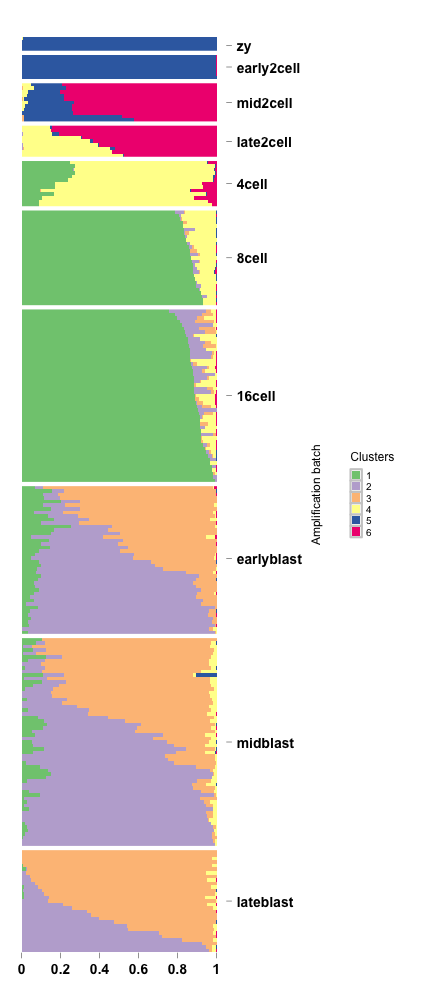
\includegraphics[width=3in,height=7in]{figure/plot_topic_deng-1} 

\end{knitrout}
\end{center}
\end{figure}

In the above plot, the samples in each batch have been sorted by the proportion of the most representative cluster. One can also use \begin{verb} order_sample=FALSE \end{verb} for the un-ordered version, which retains the order as in the data.

Now we perform for GTEx V6 data for brain samples for \Robject{k}=4.

\begin{knitrout}
\definecolor{shadecolor}{rgb}{0.969, 0.969, 0.969}\color{fgcolor}\begin{kframe}
\begin{alltt}
\hlstd{omega} \hlkwb{<-} \hlkwd{read.table}\hlstd{(}\hlstr{"../data/omega_cis_genes_brain_2.txt"}\hlstd{,}
                    \hlkwc{header} \hlstd{=} \hlnum{TRUE}\hlstd{,} \hlkwc{sep} \hlstd{=} \hlstr{" "}\hlstd{,}
                    \hlkwc{stringsAsFactors} \hlstd{=} \hlnum{FALSE}\hlstd{)}
\hlkwd{dim}\hlstd{(omega)}
\end{alltt}
\begin{verbatim}
## [1] 1259    4
\end{verbatim}
\begin{alltt}
\hlkwd{colnames}\hlstd{(omega)} \hlkwb{<-} \hlkwd{c}\hlstd{(}\hlnum{1}\hlopt{:}\hlkwd{NCOL}\hlstd{(omega))}

\hlstd{tissue_labels} \hlkwb{<-} \hlstd{gtex.meta_data[,}\hlnum{3}\hlstd{];}


\hlstd{annotation} \hlkwb{<-} \hlkwd{data.frame}\hlstd{(}
    \hlkwc{sample_id} \hlstd{=} \hlkwd{paste0}\hlstd{(}\hlstr{"X"}\hlstd{,} \hlnum{1}\hlopt{:}\hlkwd{length}\hlstd{(tissue_labels)),}
    \hlkwc{tissue_label} \hlstd{=} \hlkwd{factor}\hlstd{(tissue_labels,}
                          \hlkwc{levels} \hlstd{=} \hlkwd{rev}\hlstd{(}\hlkwd{unique}\hlstd{(tissue_labels) ) ) );}

\hlstd{cols} \hlkwb{<-} \hlkwd{c}\hlstd{(}\hlstr{"blue"}\hlstd{,} \hlstr{"darkgoldenrod1"}\hlstd{,} \hlstr{"cyan"}\hlstd{,} \hlstr{"red"}\hlstd{)}
\end{alltt}
\end{kframe}
\end{knitrout}

\begin{figure}[htp]
\begin{center}
\begin{knitrout}
\definecolor{shadecolor}{rgb}{0.969, 0.969, 0.969}\color{fgcolor}\begin{kframe}
\begin{alltt}
\hlkwd{StructureGGplot}\hlstd{(}\hlkwc{omega} \hlstd{= omega,}
                \hlkwc{annotation}\hlstd{= annotation,}
                \hlkwc{palette} \hlstd{= cols,}
                \hlkwc{yaxis_label} \hlstd{=} \hlstr{""}\hlstd{,}
                \hlkwc{order_sample} \hlstd{=} \hlnum{TRUE}\hlstd{,}
                \hlkwc{split_line} \hlstd{=} \hlkwd{list}\hlstd{(}\hlkwc{split_lwd} \hlstd{=} \hlnum{.4}\hlstd{,}
                                  \hlkwc{split_col} \hlstd{=} \hlstr{"white"}\hlstd{),}
                \hlkwc{axis_tick} \hlstd{=} \hlkwd{list}\hlstd{(}\hlkwc{axis_ticks_length} \hlstd{=} \hlnum{.1}\hlstd{,}
                                 \hlkwc{axis_ticks_lwd_y} \hlstd{=} \hlnum{.1}\hlstd{,}
                                 \hlkwc{axis_ticks_lwd_x} \hlstd{=} \hlnum{.1}\hlstd{,}
                                 \hlkwc{axis_label_size} \hlstd{=} \hlnum{7}\hlstd{,}
                                 \hlkwc{axis_label_face} \hlstd{=} \hlstr{"bold"}\hlstd{))}
\end{alltt}
\end{kframe}
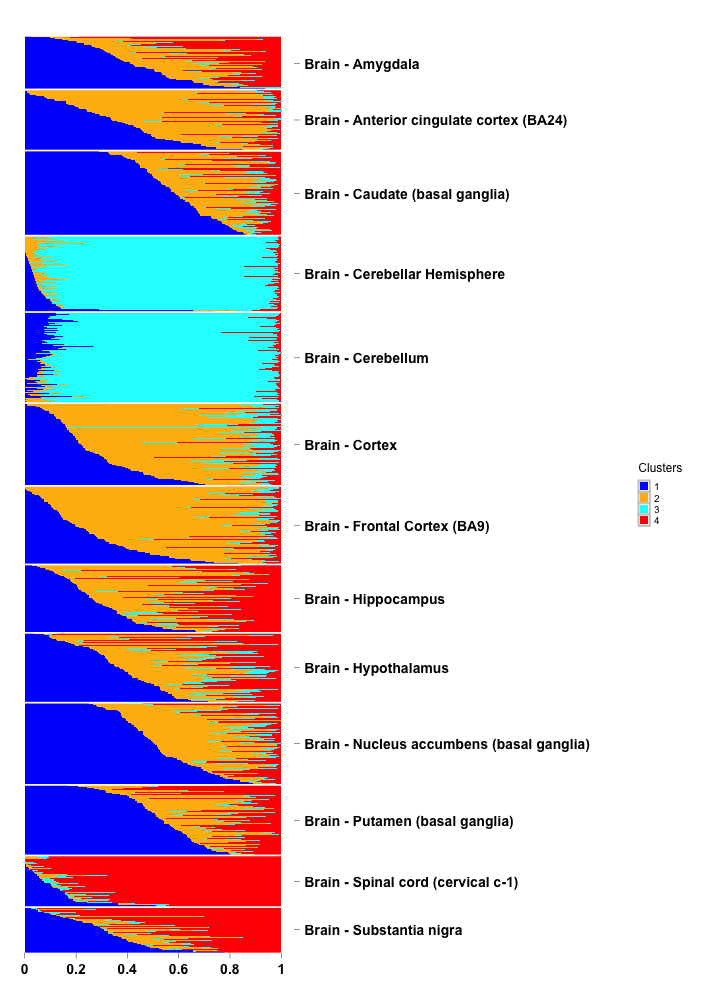
\includegraphics[width=5in,height=7in]{figure/plot_topic_gtex-1} 

\end{knitrout}
\end{center}
\end{figure}

\clearpage

\section{Cluster Annotations}

We extract the top genes driving each cluster using the \begin{verb} ExtractTopFeatures() \end{verb} functionality of the \CountClust{} package.

\begin{knitrout}
\definecolor{shadecolor}{rgb}{0.969, 0.969, 0.969}\color{fgcolor}\begin{kframe}
\begin{alltt}
\hlstd{theta_mat} \hlkwb{<-} \hlstd{MouseDeng2014.topicFit}\hlopt{$}\hlstd{clust_6}\hlopt{$}\hlstd{theta;}
\hlstd{top_features} \hlkwb{<-} \hlkwd{ExtractTopFeatures}\hlstd{(theta_mat,} \hlkwc{top_features}\hlstd{=}\hlnum{100}\hlstd{,}
                                   \hlkwc{method}\hlstd{=}\hlstr{"poisson"}\hlstd{,} \hlkwc{options}\hlstd{=}\hlstr{"min"}\hlstd{);}
\hlstd{gene_list} \hlkwb{<-} \hlkwd{do.call}\hlstd{(rbind,} \hlkwd{lapply}\hlstd{(}\hlnum{1}\hlopt{:}\hlkwd{dim}\hlstd{(top_features)[}\hlnum{1}\hlstd{],}
                        \hlkwa{function}\hlstd{(}\hlkwc{x}\hlstd{) deng.gene_names[top_features[x,]]))}
\end{alltt}
\end{kframe}
\end{knitrout}

We tabulate the top 5 genes for the 6 clusters.

\begin{knitrout}
\definecolor{shadecolor}{rgb}{0.969, 0.969, 0.969}\color{fgcolor}\begin{kframe}
\begin{alltt}
\hlkwd{library}\hlstd{(xtable)}
\hlkwd{xtable}\hlstd{(gene_list[,}\hlnum{1}\hlopt{:}\hlnum{5}\hlstd{])}
\end{alltt}
\end{kframe}
\end{knitrout}

\begin{table}[ht]
\centering
\begin{tabular}{rlllll}
  \hline
 & 1 & 2 & 3 & 4 & 5 \\
  \hline
1 & Timd2 & Isyna1 & Alppl2 & Pramel5 & Hsp90ab1 \\
  2 & Upp1 & Tdgf1 & Aqp8 & Fabp5 & Tat \\
  3 & Actb & Krt18 & Fabp3 & Id2 & Tspan8 \\
  4 & Rtn2 & Ebna1bp2 & Zfp259 & Nasp & Cenpe \\
  5 & LOC100502936 & Bcl2l10 & Tcl1 & E330034G19Rik & Oas1d \\
  6 & Obox3 & Zfp352 & Gm8300 & Usp17l5 & BB287469 \\
   \hline
\end{tabular}
\end{table}

\begin{knitrout}
\definecolor{shadecolor}{rgb}{0.969, 0.969, 0.969}\color{fgcolor}\begin{kframe}
\begin{alltt}
\hlstd{theta_mat} \hlkwb{<-} \hlkwd{as.matrix}\hlstd{(}\hlkwd{read.table}\hlstd{(}\hlstr{"../data/theta_cis_genes_brain_2.txt"}\hlstd{));}
\hlstd{top_features} \hlkwb{<-} \hlkwd{ExtractTopFeatures}\hlstd{(theta_mat,} \hlkwc{top_features}\hlstd{=}\hlnum{100}\hlstd{,}
                                   \hlkwc{method}\hlstd{=}\hlstr{"poisson"}\hlstd{,} \hlkwc{options}\hlstd{=}\hlstr{"min"}\hlstd{);}
\hlstd{gene_list} \hlkwb{<-} \hlkwd{do.call}\hlstd{(rbind,} \hlkwd{lapply}\hlstd{(}\hlnum{1}\hlopt{:}\hlkwd{dim}\hlstd{(top_features)[}\hlnum{1}\hlstd{],}
                        \hlkwa{function}\hlstd{(}\hlkwc{x}\hlstd{) gtex.gene_names[top_features[x,]]))}
\end{alltt}
\end{kframe}
\end{knitrout}

The top 3 genes (ensemble IDs) driving the 4 clusters in the GTEx V6 brain data

\begin{knitrout}
\definecolor{shadecolor}{rgb}{0.969, 0.969, 0.969}\color{fgcolor}\begin{kframe}
\begin{alltt}
\hlkwd{library}\hlstd{(xtable)}
\hlkwd{xtable}\hlstd{(gene_list[,}\hlnum{1}\hlopt{:}\hlnum{3}\hlstd{])}
\end{alltt}
\end{kframe}
\end{knitrout}

\begin{table}[ht]
\centering
\begin{tabular}{rlll}
  \hline
 & 1 & 2 & 3 \\
  \hline
  1 & ENSG00000120885.15 & ENSG00000130203.5 & ENSG00000131771.9 \\
  2 & ENSG00000171617.9 & ENSG00000160014.12 & ENSG00000154146.8 \\
  3 & ENSG00000112139.10 & ENSG00000139899.6 & ENSG00000008710.13 \\
  4 & ENSG00000197971.10 & ENSG00000266844.1 & ENSG00000237973.1 \\
   \hline
\end{tabular}
\end{table}

\section{Supplementary analysis}



Extracting the non-ERCC genes satisfying some quality measures.



We filter the metadata likewise







\begin{figure}[htp]
\begin{center}

\end{center}
\end{figure}

In the above plot, the samples within each batch is sorted by the proportion of representedness of the principal cluster driving it. One can use \begin{verb} order_sample=FALSE \end{verb} to retain the order of the samples as in the data.

\begin{figure}[htp]
\begin{center}

\end{center}
\end{figure}

\begin{thebibliography}{1}

\bibitem{Pritchard2000}
Pritchard, Jonathan K., Matthew Stephens, and Peter Donnelly.
\newblock Inference of population structure using multilocus genotype data.
\newblock {\textit{Genetics}}. 155.2,  945-959, 200.

\bibitem{Rosenberg2002}
Rosenberg NA, Pritchard JK,  Weber JL, Cann HM,  Kidd KK,  Zhivotovsky LA,  Feldman MW.
\newblock The genetic structure of human populations.
\newblock {\textit{Science}}. 298,  2381-2385, 2002.

\bibitem{Blei2003}
Blei DM,  Ng AY, Jordan MI.
\newblock Latent Dirichlet Allocation.
\newblock {\textit{J. Mach. Learn. Res.}}. 3, 993-1022, 2003.

\bibitem{Taddy2012}
Matt Taddy.
\newblock On Estimation and Selection for Topic Models.
\newblock \textit{AISTATS 2012, JMLR W\&CP 22}.(maptpx R package), 2012.

\bibitem{Jaitin2014}
Jaitin DA,  Kenigsberg E et al.
\newblock Massively Parallel Single-Cell RNA-Seq for Marker-Free Decomposition of Tissues into Cell Types.
\newblock {\textit{Science}}. 343 (6172) 776-779, 2014.

\bibitem{Deng2014}
Deng Q,  Ramskold D,  Reinius B,  Sandberg R.
\newblock Single-Cell RNA-Seq Reveals Dynamic, Random Monoallelic Gene Expression in Mammalian Cells.
\newblock {\textit{Science}}.  343 (6167) 193-196, 2014.

\bibitem{GTEX2013}
The GTEx Consortium.
\newblock The Genotype-Tissue Expression (GTEx) project.
\newblock {\textit{Nature genetics}}. 45(6): 580-585. doi:10.1038/ng.2653, 2013.

\end{thebibliography}

% \bibliography{CountClust/REFERENCES}

\section{Session Info}

\begin{knitrout}
\definecolor{shadecolor}{rgb}{0.969, 0.969, 0.969}\color{fgcolor}\begin{kframe}
\begin{alltt}
\hlkwd{sessionInfo}\hlstd{()}
\end{alltt}
\begin{verbatim}
## R version 3.2.2 (2015-08-14)
## Platform: x86_64-apple-darwin13.4.0 (64-bit)
## Running under: OS X 10.10.5 (Yosemite)
## 
## locale:
## [1] en_US.UTF-8/en_US.UTF-8/en_US.UTF-8/C/en_US.UTF-8/en_US.UTF-8
## 
## attached base packages:
## [1] parallel  stats     graphics  grDevices utils     datasets  methods  
## [8] base     
## 
## other attached packages:
## [1] cowplot_0.6.0                        reshape2_1.4.1                      
## [3] ggplot2_2.0.0                        GTExV6Brain_0.0.1                   
## [5] singleCellRNASeqMouseDeng2014_0.99.0 Biobase_2.30.0                      
## [7] BiocGenerics_0.16.1                  CountClust_0.1.0                    
## [9] knitr_1.12.3                        
## 
## loaded via a namespace (and not attached):
##  [1] Rcpp_0.12.3        digest_0.6.9       plyr_1.8.3         grid_3.2.2        
##  [5] gtable_0.1.2       formatR_1.2.1      magrittr_1.5       scales_0.3.0      
##  [9] evaluate_0.8       highr_0.5.1        stringi_1.0-1      labeling_0.3      
## [13] BiocStyle_1.8.0    RColorBrewer_1.1-2 tools_3.2.2        stringr_1.0.0     
## [17] munsell_0.4.2      colorspace_1.2-6
\end{verbatim}
\end{kframe}
\end{knitrout}

\end{document}
